% Preamble
% ---
\documentclass[a4paper]{article}

% Packages
% ---
\usepackage{bm}
\usepackage[spanish,es-nodecimaldot]{babel}
\usepackage[utf8]{inputenc}
\usepackage[T1]{fontenc}
\usepackage{parskip}
\usepackage{fancyhdr}
\usepackage{mathtools}
\usepackage{amsmath}
\usepackage[htt]{hyphenat}
\usepackage{capt-of}
\usepackage{graphicx}
\graphicspath{ {./images/} }
\usepackage{xcolor}
\usepackage{listings}

% Coding sections
% ---
\definecolor{codegreen}{rgb}{0,0.6,0}
\definecolor{codegray}{rgb}{0.5,0.5,0.5}
\definecolor{codepurple}{rgb}{0.58,0,0.82}
\definecolor{backcolour}{rgb}{0.95,0.95,0.92}
 
\lstdefinestyle{mystyle}{
    backgroundcolor=\color{backcolour},   
    commentstyle=\color{codegreen},
    keywordstyle=\color{magenta},
    numberstyle=\tiny\color{codegray},
    stringstyle=\color{codepurple},
    basicstyle=\ttfamily\footnotesize,
    breakatwhitespace=false,         
    breaklines=true,                 
    captionpos=b,                    
    keepspaces=true,                 
    numbers=left,                    
    numbersep=5pt,                  
    showspaces=false,                
    showstringspaces=false,
    showtabs=false,                  
    tabsize=2
}
 
\lstset{style=mystyle}

% Pagestyles
% ---
\pagestyle{fancy}
\rhead{Roselló Beneitez, N. U.; Roselló Oviedo, M.}
\lhead{APR: Práctica sobre MGP}
\fancyfoot[C]{\thepage}

% Main
% ---
\begin{document}

\author{Roselló Beneitez, N. U.; Roselló Oviedo, M.}
\title{APR: Práctica sobre Modelos Gráficos Probabilísticos}
\date{6 de Enero de 2020}
\maketitle{}
\thispagestyle{empty}

\newpage
\tableofcontents
\listoffigures

\newpage
\section{Descripción de la práctica}
\quad En esta práctica se ha hecho uso de la librería \textit{BNT} (\textit{Bayes Net Toolbox}) implementada en \textit{matlab} con el fin de trabajar con redes bayesianas, un subconjunto de los modelos gráficos visto en teoría.

\quad En primer lugar, se han hecho experimentos con una red de nodos booleanos que representa un césped que puede estar húmedo por causa del riego y/o la lluvia, disponiendo también de un nodo representando si el cielo se encuentra nublado.

\begin{center}
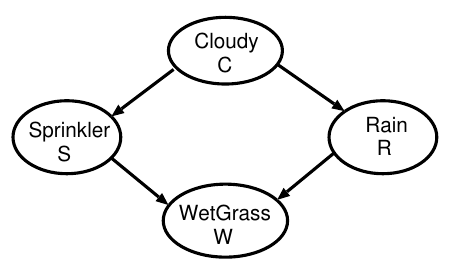
\includegraphics[width=200px]{4_ejA}
\captionof{figure}{Red bayesiana para el modelo \textit{Sprinkler}.}
\end{center}
$ \\ $

\quad Para el segundo ejercicio, hemos trabajado con la red vista en los ejemplos de la teoría representando el diagnóstico de cáncer de pulmón y/o disnea en un paciente sometido a rayos X que puede ser o no fumador y puede haber sufrido o no de polución.

\begin{center}
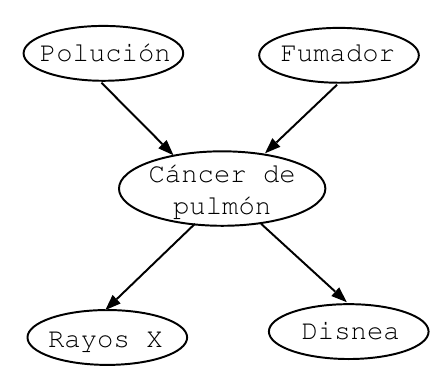
\includegraphics[width=200px]{4_ejB}
\captionof{figure}{Red bayesiana para el modelo \textit{Cáncer de pulmón}.}
\end{center}

\section{Ejercicio A}
\quad En este ejercicio se han comparado los resultados del aprendizaje a partir de datos completos (izquierda) e incompletos (derecha):

    \begin{table*}[h!]
      \noindent \begin{minipage}{.45\columnwidth}
        \begin{lstlisting}[language=octave]
		Datos completos
		W:
		1 1 : 1.0000 0.0000 
		2 1 : 0.0556 0.9444 
		1 2 : 0.0435 0.9565 
		2 2 : 0.0000 1.0000 
		S:
		1 : 0.5532 0.4468 
		2 : 0.9057 0.0943 
		R:
		1 : 0.7234 0.2766 
		2 : 0.2264 0.7736 
		C:
		1 : 0.4700 
		2 : 0.5300 
		\end{lstlisting}
      \end{minipage}\hfill
      \begin{minipage}{.6\columnwidth}
      	\begin{lstlisting}[language=octave, xleftmargin=1cm, xrightmargin=1cm]
		Datos incompletos
		W:
		1 1 : 0.9998 0.0002 
		2 1 : 0.0136 0.9864 
		1 2 : 0.1177 0.8823 
		2 2 : 0.0048 0.9952 
		S:
		1 : 0.5556 0.4444 
		2 : 0.9999 0.0001 
		R:
		1 : 0.5518 0.4482 
		2 : 0.2445 0.7555 
		C:
		1 : 0.5425 
		2 : 0.4575 
		\end{lstlisting}
      \end{minipage}
    \end{table*}
\begin{center}
\captionof{figure}{Resultados con datos completos e incompletos para la red bayesiana del modelo \textit{Sprinkler}.}
\end{center}

\quad Los resultados de los dos conjuntos de datos son muy parecidos. La única diferencia significativa observable (mayor al 10\%) está en los valores de \textit{lluvioso} (R) para el valor \textit{falso} (no llueve): cuando no está nublado, la probabilidad de que no llueva es del 55.18\% en los datos incompletos, mientras que esta misma probabilidad es del 72.34\% para los datos completos.

\quad Planteamos dos hipótesis para justificar este fenómeno: o bien se han ocultado muchos valores de \textit{lluvioso} dado un valor \textit{falso} de \textit{nublado} ($C$), en cuyo caso la red bayesiana no sabría si clasificar las muestras en verdadero o falso; o bien se han ocultado muchos de los valores \textit{nublado = falso} y algunos de los valores \textit{nublado = verdadero}, por lo que los valores de \textit{lluvioso} dado \textit{nublado = falso} podrían tomarse como la distribución \textit{a priori} de \textit{lluvioso}.

\quad Para seguir este razonamiento, cabe mencionar que si se oculta el valor de \textit{nublado} para todas las muestras (que son equiprobables), la probabilidad de \textit{lluvioso = verdadero} sería igual (o bastante parecida, como es el caso) a la probabilidad de \textit{lluvioso = falso}.

\quad Ambos razonamientos se basan en el hecho de que faltan muestras que tengan los valores de \textit{nublado = falso} o de \textit{lluvioso = falso}, pudiendo darse también una combinación de ambos.
\newpage
\section{Ejercicio B}
\quad El script \textit{matlab} para la red de diagnóstico de cáncer de pulmón se adjuntará, comentado y listo para su ejecución, junto con esta memoria. Mediante su utilización, se ha podido responder a las siguientes cuestiones:

\begin{itemize} 
\item ¿Cuál es la probabilidad de que un paciente no fumador no tenga cáncer de pulmón si la radiografía ha dado un resultado negativo pero sufre disnea?

El resultado obtenido por \textit{matlab} tras programar la red e insertar las evidencias es:

\[ P \left( C = n | F = n, X = n, D = s \right) = 0.9989 = 99.89\% \]

Podemos comprobar dicho resultado manualmente. A partir de la estructura de la red sabemos que:

\[ P(P, F, C, X, D) = P(P)\,P(F)\,P(C\,|\,P,F)\,P(X\,|\,C)\,P(D\,|\,C) \]

Por tanto, se puede deducir:

{\small \[ \begin{aligned}
&P(C\,|\,F,X,D) = \dfrac{P(C,F,X,D)}{P(F,X,D)} \\
&=\dfrac{ \sum\limits_{p\prime \in \lbrace b, a \rbrace} P(P=p\prime )\,P(F)\,P(C\,|\,P=p\prime ,F)\,P(X\,|\,C)\,P(D\,|\,C)}{ \sum\limits_{c \in \lbrace n, p \rbrace} \sum\limits_{p\prime \in \lbrace b, a \rbrace} P(P=p\prime )\,P(F)\,P(C=c\,|\,P=p\prime ,F)\,P(X\,|\,C=c)\,P(D\,|\,C=c)} \\
&= \dfrac{ P(X\,|\,C)\,P(D\,|\,C) \sum\limits_{p\prime \in \lbrace b, a \rbrace} P(P=p\prime )\,P(C\,|\,P=p\prime ,F)}{ \sum\limits_{c \in \lbrace n, p \rbrace} \left( P(X\,|\,C=c)\,P(D\,|\,C=c) \sum\limits_{p\prime \in \lbrace b, a \rbrace} P(P=p\prime )\,P(C=c\,|\,P=p\prime ,F) \right) } \end{aligned}  \]}

Aplicado a nuestro caso particular:
{\small \[ \begin{aligned}
&P \left( C = n | F = n, X = n, D = s \right) \\
&=\dfrac{ P(X=n\,|\,C=n)\,P(D=s\,|\,C=n) \sum\limits_{p\prime \in \lbrace b, a \rbrace} P(P=p\prime )\,P(C=n\,|\,P=p\prime ,F=n)}{ \sum\limits_{c \in \lbrace n, p \rbrace} \left( P(X=n\,|\,C=c)\,P(D=s\,|\,C=c) \sum\limits_{p\prime \in \lbrace b, a \rbrace} P(P=p\prime )\,P(C=c\,|\,P=p\prime ,F=n) \right) } \\
&= \dfrac{0.8 \cdot 0.3 \cdot (0.9 \cdot 0.999+0.1 \cdot 0.95)} {0.1 \cdot 0.65 \cdot (0.9 \cdot 0.001 + 0.1 \cdot 0.05) + 0.8 \cdot 0.3 \cdot (0.9 \cdot 0.999+0.1 \cdot 0.95) } \\
&= 0.998395 = 99.84\% \approx 99.89 \% \end{aligned} \]}



\item ¿Cuál es la explicación más probable de que un paciente sufra cáncer de pulmón?
\[ \lbrace \left( 1 \right) \rbrace \quad \lbrace \left( 2 \right) \rbrace \quad \lbrace \left( 2 \right) \rbrace \quad \lbrace \left( 3 \right) \rbrace \quad \lbrace \left( 2 \right) \rbrace \]
Lo cual se traduce en: polución \textbf{baja}, fumador \textbf{sí}, cáncer \textbf{positivo}, rayos X \textbf{positivo} y disnea \textbf{sí}. El log-verosimilitud de esta explicación es de $-5.0925$, esto es, una probabilidad de $e^{-5.0925}=0.0061=0.61\%$.
\end{itemize}

\section{Conclusiones}
\quad Las redes bayesianas nos permiten representar gráficamente y de una forma compacta distribuciones de probabilidad conjunta. Su capacidad de aprendizaje e inferencia nos manifiesta su utilidad como herramienta potencial para múltiples aplicaciones como pueden ser las predicciones o el diagnóstico médico (como hemos visto con estos ejemplos); así como para otros campos como pueden ser la visión por computador o el procesado de lenguajes naturales.

\end{document}
